\documentclass[10pt]{beamer}
%\usetheme{Boadilla}
%\usecolortheme{beaver}
%\usepackage[latin1]{inputenc}
\useoutertheme{split}
\setbeamertemplate{navigation symbols}{}
\usefonttheme[onlymath]{serif}
\usepackage{amsmath}%
\usepackage{amsthm}%
\usepackage{amsfonts}%
\usepackage{amssymb}%
\usepackage[algo2e]{algorithm2e}
\usepackage{algorithmic}  
\usepackage{algorithm}
\usepackage{tikz}
\usepackage[english]{babel}
\usepackage{amsmath, amssymb, amsthm}
\usepackage{verbatim}
\usepackage{mathrsfs}
%\usepackage{epstopdf}
\usepackage{graphicx}
\mode<presentation>
{
	\usetheme{CambridgeUS}
	\usecolortheme{dolphin}
	\usecolortheme{rose}
	\setbeamercovered{transparent}
}
\newcommand{\mrel}{\mathrel{\bigcirc}}
%\usepackage[onehalfspacing]{setspace}
%\setbeamertemplate{footline}[frame number]
\DeclareMathOperator*{\Bigcdot}{\scalerel*{\cdot}{\bigodot}}
% Macros
\def\a{\alpha} \def\b{\beta} \def\c{\gamma} \def\d{\delta} \def\r{\rho}
\def\e{\epsilon} \def\ve{\varebsilon} \def\k{\kappa} \def\p{\pi} \def\th{\theta}
\def\l{\lambda} \def\m{\mu} \def\s{\sigma} \def\t{\tau} \def\w{\omega} \def\z{\zeta}
\def\D{\Delta} \def\G{\Gamma} \def\W{\Omega} \def\P{\Phi} \def\L{\Lambda}
\def\bdm{\begin{displaymath}} \def\edm{\end{displaymath}}
\def\bni{\begin{itemize}} \def\ei{\end{itemize}}
\def\bnen{\begin{enumerate}} \def\een{\end{enumerate}}
\def\fa{\forall}
\def\be{\begin{equation}} \def\ee{\end{equation}}
\def\fn{\footnote} \def\bn{\begin} \def\nit{\noindent}
\def\iff{\textit{~if and only if~~}}
\renewcommand*{\thefootnote}{\fnsymbol{footnote}}
% THEOREMS -------------------------------------------------------
\newtheorem{thm}{Theorem}%[section]
\newtheorem{cor}[thm]{Corollary}
\newtheorem{lem}[thm]{Lemma}
\newtheorem{prop}[thm]{Proposition}
\newtheorem{claim}{Claim}
\theoremstyle{definition}
%\newtheorem{defn}[thm]{Definition}
\theoremstyle{remark}
\newtheorem{rem}[thm]{Remark}
%%\numberwithin{equation}{section}  
 
\newcommand{\N}{\mathbb{N}}
\newcommand{\Z}{\mathbb{Z}}
\newcommand{\R}{\mathbb{R}}
\newcommand{\ls}{\left\{}
\newcommand{\rs}{\right\}}


\title[Dynamic AME Model (DAME)]{ \vspace{-.25cm} \\ Dynamic Additive and Multiplicative Effects (DAME)\\ Network Model with Application to \\the United Nations Voting Behaviors}
\author[\quad\quad  Bomin Kim, Xiaoyue Niu, and David Hunter\quad \quad]{
\quad Bomin Kim\textsuperscript{1}\and
\quad Xiaoyue Niu\textsuperscript{1}\and\\
David Hunter \textsuperscript{1}\and Xun Cao\textsuperscript{2}}
\institute{\textsuperscript{1} Department of Statistics\and \textsuperscript{2}  Department of Political Science\and  \vspace{.25cm} \small The Pennsylvania State University}

\begin{document}
 
\begin{frame}
  \titlepage
\end{frame}


\begin{frame}{Dynamic Additive and Multiplicative Effects Model}
	\bni
	\item Network regression model for symmetric discrete-time networks\\
	\vspace{0.4cm}
	\item Integration of two existing works:\\
		\vspace{0.2cm}
	 \begin{itemize}
	 	\item [1.] Model formulation: AMEN for latent factor models\\\hspace{2.5cm} (Minhas, Hoff, and Ward, 2016)\\	\vspace{0.2cm}
	\item[2.]GP Priors: Bayesian dynamic networks with time-varying predictors\\ \hspace{1.4cm} (Durante and Dunson, 2014)\\
	\end{itemize}
	\ei
\end{frame}


\begin{frame}{Model Formulation}
	\bni
	\item For $N \times N$ symmetric matrices $\mathcal{Y}=\{Y(t), t \in \mathcal{T}\}$, define $(i, j)^{th}$ entry
	 \begin{equation*}
	\begin{aligned}
	&y_{ij}(t)=X^T_{ij}(t)\beta(t)+\theta_i(t)+\theta_j(t)+{u_i(t)^TD(t)u_j(t)}+\epsilon_{ij}(t),
	\end{aligned}
	\end{equation*}
	where
	\begin{itemize}
		\item[1.] $\beta(t)$: $P-$dimensional edge covariate effects 
		\item[2.] $\theta_i(t)$ and $\theta_j(t)$: additive nodal random effects of $i$ and $j$
		\item[3.] $u_i(t)^TD(t)u_j(t)$: multiplicative random effect
		%\begin{itemize}
		%	\item[-] $D(t)$: $R \times R$ diagonal matrix
		%	\item[-] $u_i(t)$ and $u_j(t)$: $R-$dimensional vector of latent coordinates of $i$ and $j$
		%\end{itemize}
		\item[4.] $\epsilon_{ij}(t)$: random noise
	\end{itemize}\vspace{0.4cm}
	\item Each parameter has Gaussian process (GP) priors
	 \begin{equation*}
	 \begin{aligned}
	 &\beta_{p}(\cdot) \sim \mbox{GP}(0, \tau^{\beta}_pc_\beta)\mbox{ for }p = 1,...,P\\& 
	 \tau^{\beta}_p \sim \mbox{IG}(a_\beta, b_\beta) \mbox{ and } c_\beta(t, t')=f(\kappa_{\beta_p}, |t-t'|),
	 \end{aligned}
	 \end{equation*}
	 where $f()$ is Exponential or squared Exponential covariance functions.
	\ei
\end{frame}

 \begin{frame}{United Nations Voting Networks}
 	\bni
 	\item Roll-call votes in the UN General Assembly 1983-2014 (Voeten et al.,  2016)	\vspace{0.4cm}
 	\item 23 most “active” countries in international relations (Hoff, 2015)	\vspace{0.4cm}
 	\item Annual agreement network from `Yes', `No', and `Abstain'	\vspace{0.4cm}
 	\item Six relevent dyadic predictors:
 	\begin{itemize}
 		\item [1.] Intercept
 		\item [2.] log(distance)$_{ij}$
 		\item [3.] Alliance$_{ijt}$
 		\item [4.] Polity score difference$_{ijt}$
 		\item [5.] Lower trade-to-GDP ratio$_{ijt}$ (Gartzke, 2000)
 		\item [6.] Common language$_{ij}$
 	\end{itemize}
 	\ei
\end{frame}

\begin{frame}{Results: Main Effects and Random Effects}
	\begin{figure}[ht]
		\begin{center}
			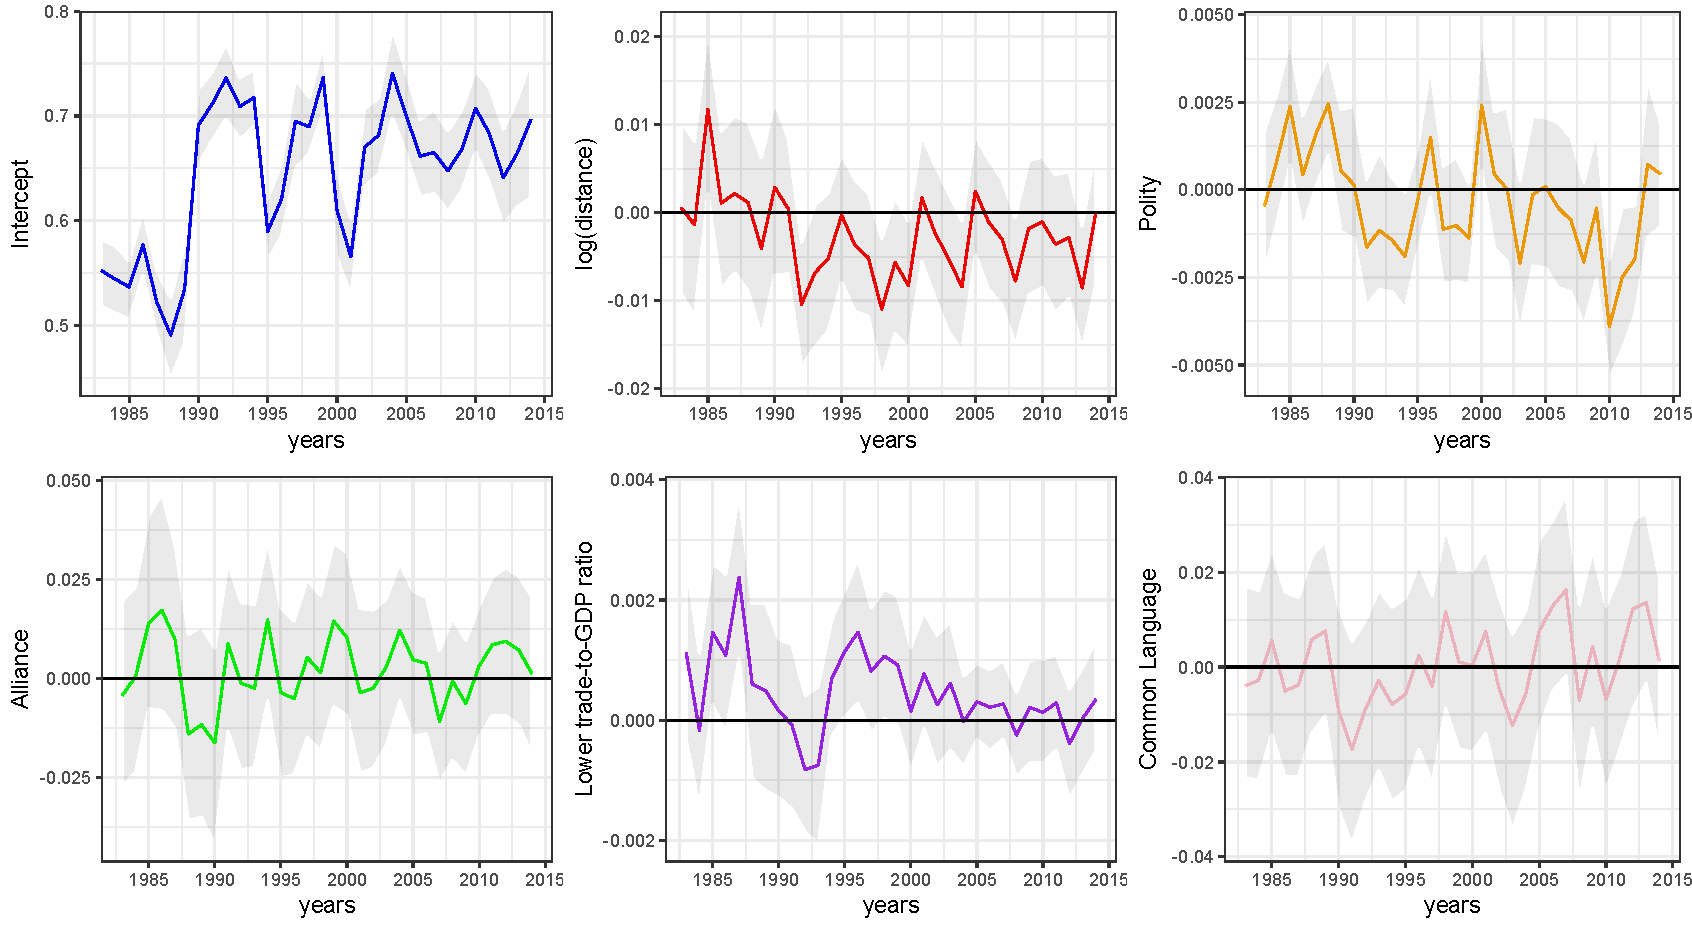
\includegraphics[width=0.6\textwidth]{betas.pdf}	
		\end{center}
	\end{figure}
		\begin{figure}[ht]
			\begin{center}
							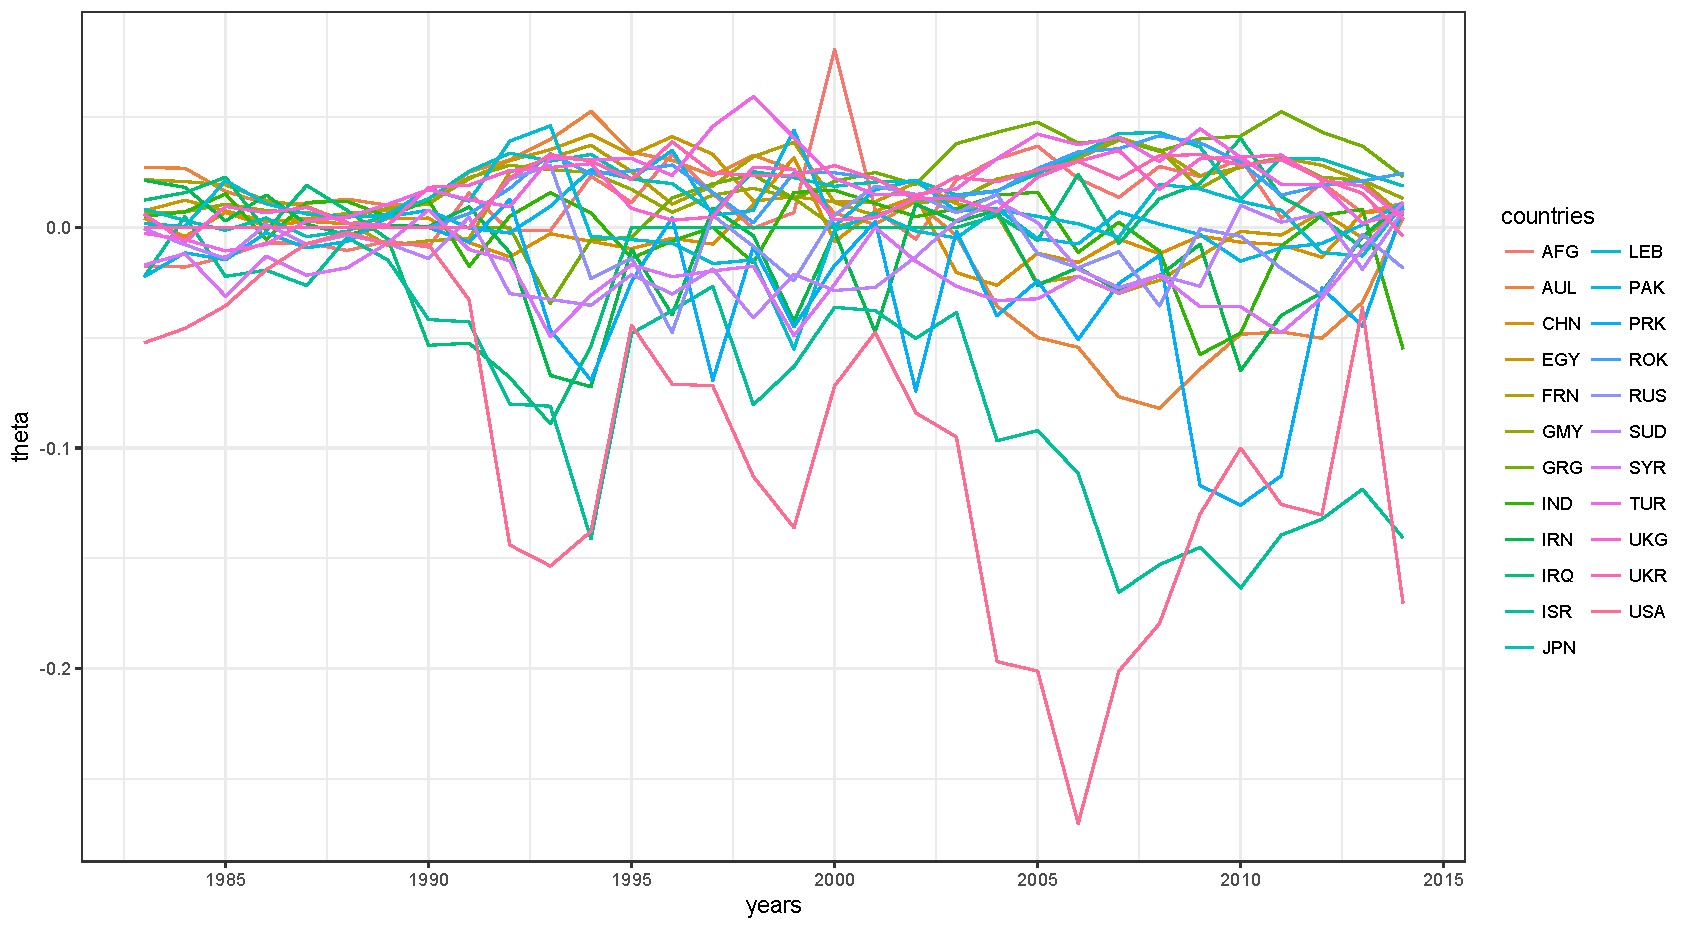
\includegraphics[width=0.5\textwidth]{theta.pdf}	
				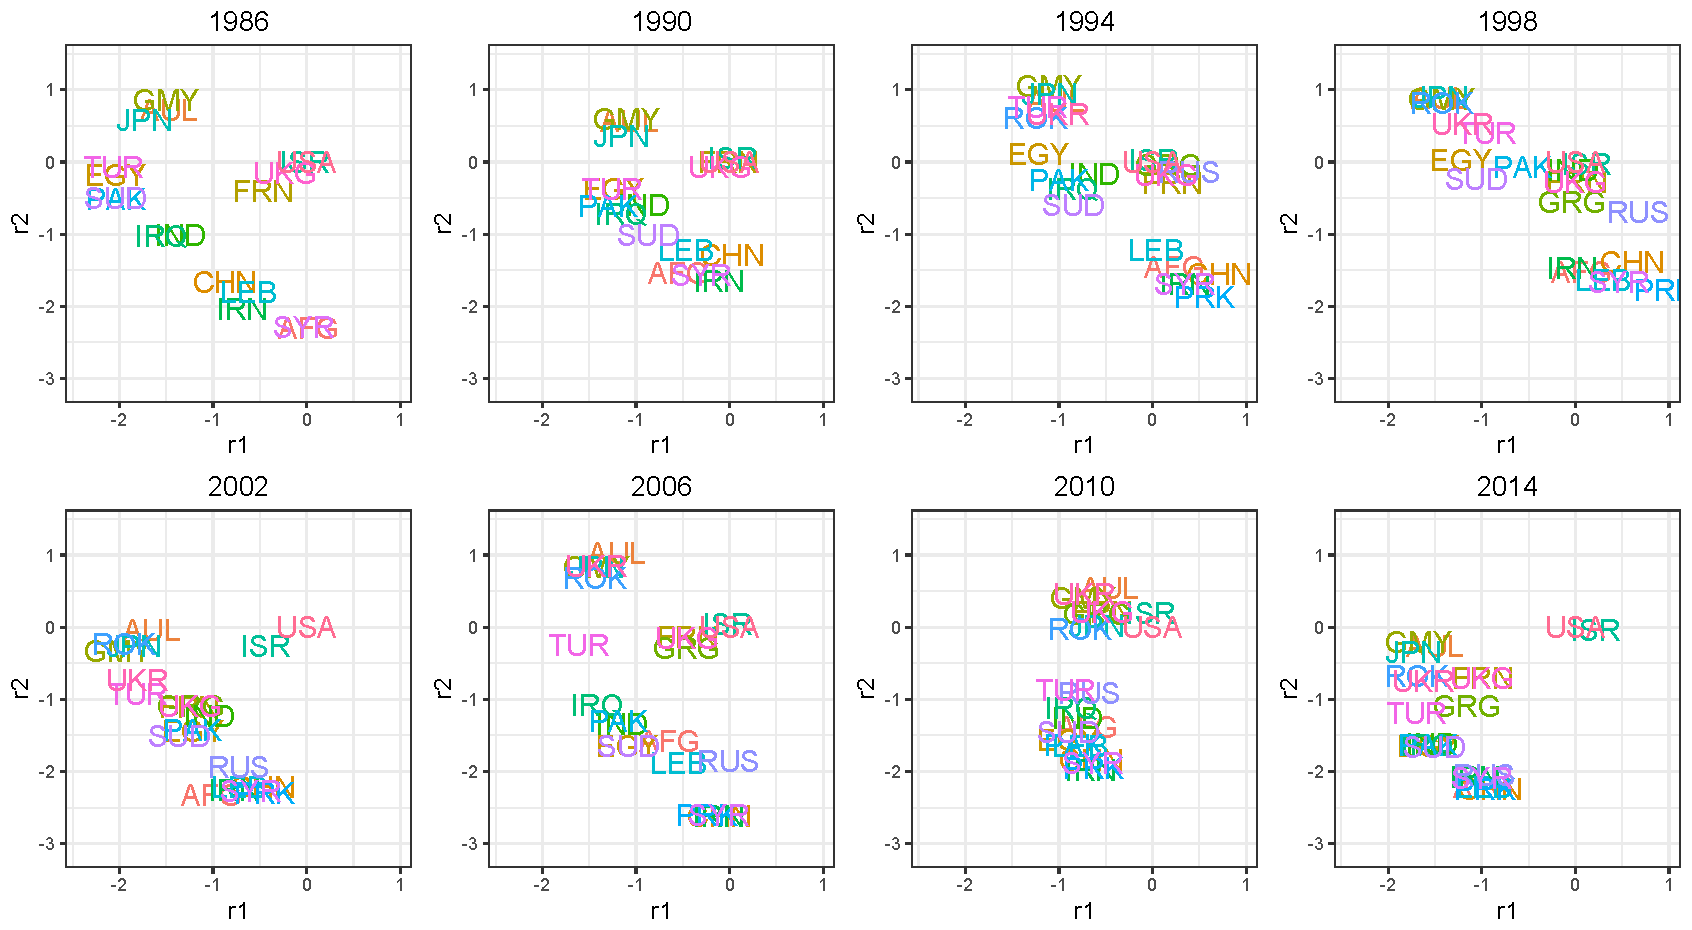
\includegraphics[width=0.5\textwidth]{UDU.pdf}	
			\end{center}
		\end{figure}
\end{frame}
\end{document}